%%%%%%%%%%%%%%%%%%%%%%%%%%%%%%%%%%%%%%%%%
% Jacobs Landscape Poster
% LaTeX Template
% Version 1.0 (29/03/13)
%
% Created by:
% Computational Physics and Biophysics Group, Jacobs University
% https://teamwork.jacobs-university.de:8443/confluence/display/CoPandBiG/LaTeX+Poster
% 
% Further modified by:
% Nathaniel Johnston (nathaniel@njohnston.ca)
%
% This template has been downloaded from:
% http://www.LaTeXTemplates.com
%
% 
% Masaryk University presentation themes were downloaded from:
% https://www.overleaf.com/gallery/tagged/muni
%
% and ported into Jacobs Landscape Poster by:
% Jumaidil Awal (ideal1st.here@googlemail.com)
% 
% Jacobs Landscape Poster License:
% CC BY-NC-SA 3.0 (http://creativecommons.org/licenses/by-nc-sa/3.0/)
%
% Masaryk University's fibeamer theme license:
% Copyright 2015  Vít Novotný <witiko@mail.muni.cz>
% Faculty of Informatics, Masaryk University (Brno, Czech Republic)
% under Latex Project Public License
%
%%%%%%%%%%%%%%%%%%%%%%%%%%%%%%%%%%%%%%%%%

%----------------------------------------------------------------------------------------
%	PACKAGES AND OTHER DOCUMENT CONFIGURATIONS
%----------------------------------------------------------------------------------------

\documentclass[final]{beamer}

\usepackage[scale=1.24]{beamerposter} % Use the beamerposter package for laying out the poster
\usepackage[font=small,skip=0pt]{caption}
%\usetheme{confposter} % Use the confposter theme supplied with this template
\usetheme[faculty=chemo]{fibeamer} % Uncomment to use Masaryk University's fibeamer theme instead.

%\setbeamercolor{block title}{fg=ngreen,bg=white} % Colors of the block titles
%\setbeamercolor{block body}{fg=black,bg=white} % Colors of the body of blocks
%\setbeamercolor{block alerted title}{fg=white,bg=dblue!70} % Colors of the highlighted block titles
%\setbeamercolor{block alerted body}{fg=black,bg=dblue!10} % Colors of the body of highlighted blocks
% Many more colors are available for use in beamerthemeconfposter.sty

%-----------------------------------------------------------
% Define the column widths and overall poster size
% To set effective sepwid, onecolwid and twocolwid values, first choose how many columns you want and how much separation you want between columns
% In this template, the separation width chosen is 0.024 of the paper width and a 4-column layout
% onecolwid should therefore be (1-(# of columns+1)*sepwid)/# of columns e.g. (1-(4+1)*0.024)/4 = 0.22
% Set twocolwid to be (2*onecolwid)+sepwid = 0.464
% Set threecolwid to be (3*onecolwid)+2*sepwid = 0.708

\newlength{\sepwid}
\newlength{\onecolwid}
\newlength{\twocolwid}
\newlength{\threecolwid}
\setlength{\paperwidth}{46.8in} % A0 width: 46.8in
\setlength{\paperheight}{33.1in} % A0 height: 33.1in
\setlength{\sepwid}{0.024\paperwidth} % Separation width (white space) between columns
\setlength{\onecolwid}{0.21\paperwidth} % Width of one column
\setlength{\twocolwid}{0.451\paperwidth} % Width of two columns
\setlength{\threecolwid}{0.678\paperwidth} % Width of three columns
%\setlength{\topmargin}{-0.5in} % Reduce the top margin size
%-----------------------------------------------------------

\usepackage{graphicx}  % Required for including images

\usepackage{booktabs} % Top and bottom rules for tables

%----------------------------------------------------------------------------------------
%	TITLE SECTION 
%----------------------------------------------------------------------------------------

\title{Solid Waste Management} % Poster title

\author{Dhwani Agarwal} % Author(s)

\institute{VJTI, Mumbai} % Institution(s)

%----------------------------------------------------------------------------------------

\begin{document}
\addtobeamertemplate{block end}{}{\vspace*{2ex}} % White space under blocks
\addtobeamertemplate{block example end}{}{\vspace*{2ex}} % White space under example blocks
\addtobeamertemplate{block alerted end}{}{\vspace*{2ex}} % White space under highlighted (alert) blocks

\setlength{\belowcaptionskip}{2ex} % White space under figures
\setlength\belowdisplayshortskip{2ex} % White space under equations
%\begin{darkframes} % Uncomment for dark theme, don't forget to \end{darkframes}
\begin{frame} % The whole poster is enclosed in one beamer frame

%==========================Begin Head===============================

  \begin{columns}
   \begin{column}{\linewidth}
    \vskip1cm
    \centering
    \usebeamercolor{title in headline}{\color{fg}\Huge{\textbf{\inserttitle}}\\[0.5ex]}
    \usebeamercolor{author in headline}{\color{fg}\Large{\insertauthor}\\[1ex]}
    \usebeamercolor{institute in headline}{\color{fg}\large{\insertinstitute}\\[1ex]}
    \vskip1cm
   \end{column}
   \vspace{1cm}
  \end{columns}
 \vspace{1cm}

%==========================End Head===============================

\begin{columns}[t] % The whole poster consists of three major columns, the second of which is split into two columns twice - the [t] option aligns each column's content to the top

\begin{column}{\sepwid}\end{column} % Empty spacer column

\begin{column}{\onecolwid} % The first column

%----------------------------------------------------------------------------------------
%	OBJECTIVES
%----------------------------------------------------------------------------------------

\begin{exampleblock}{Introduction}

Higher standards of living of ever increasing population has resulted in an increase in the quantity and variety of waste generated. It is now realized that if the waste generation continues indiscriminately then very soon it will be beyond rectification. Management of solid waste has, therefore, become very important in order to minimize the adverse effects of solid wastes. Solid waste (waste other than liquid or gaseous) can be classified as municipal, industrial, agricultural, medical, mining waste and sewage sludge.
\end{exampleblock}

%----------------------------------------------------------------------------------------
%	INTRODUCTION
%----------------------------------------------------------------------------------------

\begin{exampleblock}{Sources of Urban and Industrial Wastes}
Urban waste consists of medical waste from hospitals, municipal solid wastes from homes, offices, markets (commercial waste) small cottage units, and horticulture waste from parks, gardens, orchards etc.\\
Industrial waste consists of a large number of materials including factory rubbish, packaging material, organic wastes, acids, alkalis, scrap metal, abrasives, oils, paints, asphalt, asbestos, batteries et. 
\end{exampleblock}

%------------------------------------------------

\begin{figure}

\includegraphics[width=1\linewidth]{img/swaste.jpg}
\caption{Solid waste \smallskip https://www.britannica.com/technology/solid-waste-management}
% \captionsource{https://www.google.com/search?client=firefox-b-d&q=solid+waste+images}
\end{figure}

%----------------------------------------------------------------------------------------

\end{column} % End of the first column

\begin{column}{\sepwid}\end{column} % Empty spacer column

\begin{column}{\twocolwid} % Begin a column which is two columns wide (column 2)

\begin{columns}[t,totalwidth=\twocolwid] % Split up the two columns wide column

\begin{column}{\onecolwid}\vspace{-.74in} % The first column within column 2 (column 2.1)

%----------------------------------------------------------------------------------------
%	MATERIALS
%----------------------------------------------------------------------------------------

\begin{exampleblock}{Effects of solid waste}
\begin{itemize}
    \item Dumping allows biodegradable materials to decompose under uncontrolled and unhygienic conditions, producing foul smell.
    \item Industrial solid waste cause changes in physiochemical and biological characteristics of the soil.
    \item Toxic substances leach or percolate to contaminate ground water.
    \item Burning of waste produces dioxins, furans and polychlorinated biphenyls which have potential to cause various types of ailments including cancer.
\end{itemize}

\end{exampleblock}
\begin{exampleblock}{The 3 R's}

\textbf{Reduce - } Reduction in use of raw materials correspondingly decrease the production of waste.

\textbf{Reuse - } The refillable containers which are discarded after use can be recycled. Making rubbers rings from the discarded cycle tubes which are used by the newspaper vendors instead of rubber bands reduce the waste generation during manufacturing of rubber bands. 

\textbf{Recycle - } Recycling is the reprocessing of discarded materials into new useful products. Example) Old aluminium cans and glass bottles are melted and recast into new cans and bottles. Preparation of cellulose insulation from paper, preparation of fuel pellets from kitchen waste.
%\begin{figure}
%
\includegraphics[width=1\linewidth]{img/r.jpg}
%\caption{3 R's cycle}
%\end{figure}

\end{exampleblock}
%----------------------------------------------------------------------------------------


\end{column} % End of column 2.1
\begin{column}{\sepwid}\end{column} % Empty spacer column

\begin{column}{\onecolwid}\vspace{-.74in} % The second column within column 2 (column 2.2)

%----------------------------------------------------------------------------------------
%	METHODS
%----------------------------------------------------------------------------------------

\begin{exampleblock}{Methods for discarding waste}

\begin{enumerate}
\item \textbf{Sanitary Landfill} - Garbage is spread out in thin layers, compacted and covered with clay or plastic foam. The bottom is covered with an impermeable liner usually several layers of clay, thick plastic, and sand to avoid leaching
\begin{figure}
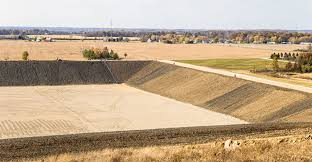
\includegraphics[width=1\linewidth]{img/landfill.jpg}
\caption{Sanitary Landfill \smallskip https://www.britannica.com/sanitary-landfill}
\end{figure}
\item \textbf{Composting} - The biodegradable yard waste (kept separate from municipal waste) is allowed to degrade or decompose in an oxygen rich medium. Manure thus formed improves the soil conditions and fertility.
\begin{figure}
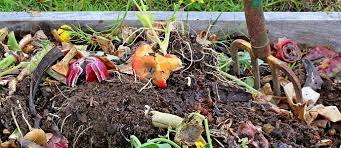
\includegraphics[width=1\linewidth]{img/compost.jpg}
\caption{Composting \smallskip https://www.recyclenow.com/composting}
\end{figure}
\item \textbf{Incineration} - Incinerators are burning plants capable of burning large amount of materials at high temperature. During incineration high levels of dioxins, furans, lead, cadmium is emitted along with fly ash. It is better to remove batteries containing heavy metals and plastic containing chlorine before burning the material.
\end{enumerate}




\end{exampleblock}

%----------------------------------------------------------------------------------------

\end{column} % End of column 2.2

\end{columns} % End of the split of column 2 - any content after this will now take up 2 columns width

%----------------------------------------------------------------------------------------
%	IMPORTANT RESULT
%----------------------------------------------------------------------------------------

%\begin{alertblock}{Important Result}
%\begin{figure}
%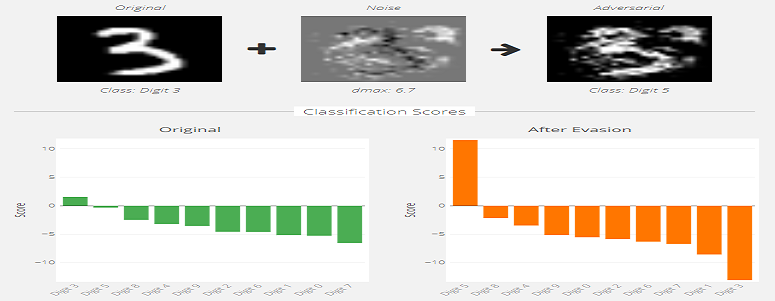
\includegraphics[width=1\linewidth]{img/result.PNG}
%\end{figure}
% Images that can be misclassified by deep-learning algorithms while being only imperceptibly distorted. evasion attacks are thus already a relevant threat in real-world application settings.

%\end{alertblock} 

%----------------------------------------------------------------------------------------

\begin{columns}[t,totalwidth=\twocolwid] % Split up the two columns wide column again

\begin{column}{\onecolwid} % The first column within column 2 (column 2.1)

%----------------------------------------------------------------------------------------
%	MATHEMATICAL SECTION
%----------------------------------------------------------------------------------------



%----------------------------------------------------------------------------------------

\end{column} % End of column 2.1
\begin{column}{\sepwid}\end{column} % Empty spacer column

\begin{column}{\onecolwid} % The second column within column 2 (column 2.2)

%----------------------------------------------------------------------------------------
%	RESULTS
%----------------------------------------------------------------------------------------



%----------------------------------------------------------------------------------------

\end{column} % End of column 2.2

\end{columns} % End of the split of column 2

\end{column} % End of the second column

\begin{column}{\sepwid}\end{column} % Empty spacer column

\begin{column}{\onecolwid} % The third column

%----------------------------------------------------------------------------------------
%	CONCLUSION
%----------------------------------------------------------------------------------------

\begin{exampleblock}{Conclusion}
There are significant issues with unauthorized waste disposal practices due to the lack of proper waste management process.
It is clear that improper waste management practices have a significant impact on the natural environment and sustainable development.
Thus it is important that solid waste management should be developed from the primary level. 
This can include, waste separation from the household level, proper storage, more efficient waste collection systems, and sustainable recovery and disposal practices.
Awareness programmes must be conducted in order to improve the knowledge about the importance of solid waste management for sound environmental development.
\begin{figure}
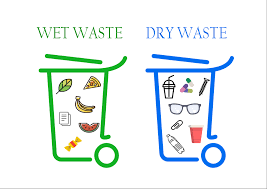
\includegraphics[width=1\linewidth]{img/conclude.png}
\caption{Waste Separation \smallskip https://www.britannica.com/technology/solid-waste-management}
\end{figure}
 
\end{exampleblock}

%----------------------------------------------------------------------------------------
%	ADDITIONAL INFORMATION
%----------------------------------------------------------------------------------------

%\begin{exampleblock}{Additional Information}

%Maecenas ultricies feugiat velit non mattis. Fusce tempus arcu id ligula varius dictum. 
%\begin{itemize}
%\item Curabitur pellentesque dignissim
%\item Eu facilisis est tempus quis
%\item Duis porta consequat lorem
%\item Duis porta consequat lorem
%\end{itemize}

%\end{exampleblock}

%----------------------------------------------------------------------------------------
%	REFERENCES
%----------------------------------------------------------------------------------------

\begin{exampleblock}{References}


\begin{thebibliography}{2}
\bibitem{} \textbf{Anubha Kaushik ans CP Kaushik}\\ Perspectives in environmental studies
\bibitem{} https://www.britannica.com/technology/

\end{thebibliography}
\end{exampleblock}

%----------------------------------------------------------------------------------------
%	ACKNOWLEDGEMENTS
%----------------------------------------------------------------------------------------

%\setbeamercolor{block title}{fg=red,bg=white} % Change the block title color

%\begin{exampleblock}{Acknowledgements}

%\small{\rmfamily{Nam mollis tristique neque eu luctus. Suspendisse rutrum congue nisi sed convallis. Aenean id neque dolor. Pellentesque habitant morbi tristique senectus et netus et malesuada fames ac turpis egestas.}} \\

%\end{exampleblock}

%----------------------------------------------------------------------------------------
%	CONTACT INFORMATION
%----------------------------------------------------------------------------------------

%\setbeamercolor{block alerted title}{fg=black,bg=norange} % Change the alert block title colors
%\setbeamercolor{block alerted body}{fg=black,bg=white} % Change the alert block body colors

%\begin{block}{Contact Information}
    
%    \begin{itemize}
 %   \item Web: \href{http://ideal1st.com/}{http://ideal1st.com/}
  %  \item Email: \href{mailto:ideal1st.here@gmail.com}{ideal1st.heregmail.com}
%   \end{itemize}
    
 %   \end{block}
    
%    \begin{tabular}{rr}
%    \hspace{0.3\linewidth} & 
\includegraphics[width=0.5\linewidth]{img/logo.png}
 %   \end{tabular}

%----------------------------------------------------------------------------------------

\end{column} % End of the third column

\begin{column}{\sepwid}\end{column} % Empty spacer column

\end{columns} % End of all the columns in the poster

\end{frame} % End of the enclosing frame
%\end{darkframes} % Uncomment for dark theme
\end{document}
